В этой главе мы воспользуемся знаниями предыдущей и получим различные эквивалентные представления данных, чтобы на практике переключаться между ними в зависимости от обстоятельств.

\subsection{Всё --- свёртка} \label{subsec:all-folds}

Вспомним, что любую рекурсивную структуру данных можно представить как неподвижную точку функтора, задающего форму (\ref{subsubsec:functor-fixpoint}).
При этом существует универсальная свёртка, катаморфизм, которая работает для произвольного функтора формы (\ref{subsubsec:recursion-schemas}):
\begin{minted}{haskell}
    cata :: Functor f => (f a -> a) -> Fix f -> a
\end{minted}

Оказывается, что с помощью катаморфизма можно получить изоморфизм между структурами данных и их свёртками:
\mintinline{haskell}|Fix f ?$\simeq$? forall a . (f a -> a) -> a|.
\begin{minted}{haskell}
    to :: Functor f => Fix f -> (forall a . (f a -> a) -> a)
    to = flip cata

    from :: (forall a . (f a -> a) -> a) -> Fix f
    from g = g In
\end{minted}

Например, следующие два списка эквивалентны (все конструкторы \mintinline{haskell}{In} заменяем на данную алгебру):
\begin{minted}{haskell}
    data List elem rec = Nil | Cons elem rec

    xs1 :: Fix (List Int)
    xs1 = In (Cons 1 (In (Cons 2 (In (Cons 3 (In Nil))))))

    xs2 :: (List Int a -> a) -> a
    xs2 = \alg -> alg (Cons 1 (alg (Cons 2 (alg (Cons 3 (alg Nil))))))

    ghci> xs2 @Int \case Nil -> 0; Cons x acc -> x + acc
    6
\end{minted}

Теперь избавимся от функтора формы.
Это нерекурсивный тип, который можно представить в канонической форме (см.~\ref{subsubsec:type-algebra}):
\[
    f\ap a \iso \sum_{i}\prod_{j} (t_{ij}\ap a)
\]
Тогда алгебра может быть записана следующим образом:
\[
    f\ap a\to a\iso a^{\sum_{i}\prod_{j} (t_{ij}\ap a)} \iso \prod_{i}a^{\prod_{j} (t_{ij}\ap a)}
\]
Остались произведения, от которых можно избавиться с помощью каррирования, и получить \vocab{финальное кодирование} структуры данных\footnote{Финальным такое кодирование называется по историческим причинам. Казалось, что оно двойственно инициальному и является терминальным (финальным) объектом категории интерпретаций. Однако, с категорной точки зрения, это тоже инициальный объект.}.
Например, для списка имеем:
\begin{align*}
    \text{\mintinline{haskell}{(List elem a -> a) -> a}}
    \iso a^{\displaystyle a^{\displaystyle 1 + elem\times a}}
    \iso a^{\displaystyle a\times a^{\displaystyle elem\times a}}
    \iso \left( a^{\displaystyle a} \right)^{\displaystyle \left(\left( a^{\displaystyle a}\right)^{\displaystyle elem}\right)} \\
    \iso \text{\mintinline{haskell}{a -> (elem -> a -> a) -> a}}
\end{align*}

Мы получили не что иное, как список Чёрча\footnote{\url{https://en.wikipedia.org/wiki/Church_encoding}}\footnote{\url{https://okmij.org/ftp/tagless-final/course/Boehm-Berarducci.html}}.
Структуру данных, без единого конструктора!\footnote{На самом деле в этом нет ничего удивительного, если вспомнить, что функции первого класса представляются как замыкания, содержащие данные. Мы получили тот же односвязный список, только на замыканиях.}
Перепишем знакомый нам список ещё раз:
\begin{minted}{haskell}
    xs3 :: a -> (Int -> a -> a) -> a
    xs3 = \ini f -> f 1 (f 2 (f 3 ini))
\end{minted}

\begin{task}
    Какая знакомая вам стандартная функция работы со списками по \mintinline{haskell}{data} списку возвращает список Чёрча?
\end{task}

Попробуем интуитивно понять, что это всё значит.
Заметим, что список Чёрча принимает функции, соответствующие веткам паттерн-матчинга или аргументам сворачивающей функции.
Вместо конструкторов же сразу вызываются соответствующие функции.
То есть, вместо того, чтобы создать структуру данных и доставить её к месту деконструирования (паттерн-матчингу), мы \point{доставляем место деконструирования к месту конструирования} и оказывается, что ничего конструировать по итогу и не надо.

Стоит отметить, что изоморфизм \mintinline{haskell}|Fix f ?$\simeq$? forall d . (f d -> d) -> d|, на котором основывается этот раздел, является обобщением изоморфизма \mintinline{haskell}{a ?$\sim$? forall r . (a -> r) -> r} (при \mintinline{haskell}{f = Const a}), который является основой CPS трансформации, рассматриваемой нами далее в~\ref{sec:continuations}.

\subsubsection{Deforestation \& fusion} \label{subsubsec:deforestation-fusion}

В функциональном программировании мы строим новые функции путём композирования имеющихся, более простых, функций.
Этот подход позволяет переиспользовать реализованную функциональность, снижая сложность кода и вероятность ошибок.
Однако, он может приводить к излишним накладным расходам на аллокацию и деконструирование промежуточных структур данных.

Например, сравните следующие две реализации.
Первая предпочтительна с точки зрения качества кода, однако она порождает промежуточный список во время работы:
\begin{minted}{haskell}
    all p xs = and (map p xs)
    -- или fused версия
    all p [] = []
    all p (x:xs) = p x && all p xs
\end{minted}

Очевидно, это задача оптимизирующего компилятора превращать хороший код с абстракциями в быстрый код.
Оптимизация, избавляющая программы от (промежуточных) структур данных (деревьев) называется \vocab{дефорестацией (deforestation)}.
В результате две функции, как говорят, ``сплавляются'' --- fuse.

Термин и первый дефорестирующий алгоритм был предложен Philip Wadler~\cite{wadler1988deforestation}, он основан на нескольких простых правилах переписывания и агрессивном инлайнинге (см. примеры работы на рис.~\ref{fig:deforestation-examples}).
Однако, этот алгоритм может приводить к экспоненциальному разбуханию кода и имеет шанс не завершится при наличии рекурсивных вызовов\footnote{Дефорестация является частным случаем суперкомпиляции~\cite{supercomp}, которая в свою очередь является обобщеним большого количества компиляторных оптимизаций.}.
Чтобы алгоритм завершался программы должны быть написаны в некоторой строгой форме под названием treeless.

\begin{figure}
    \centering
    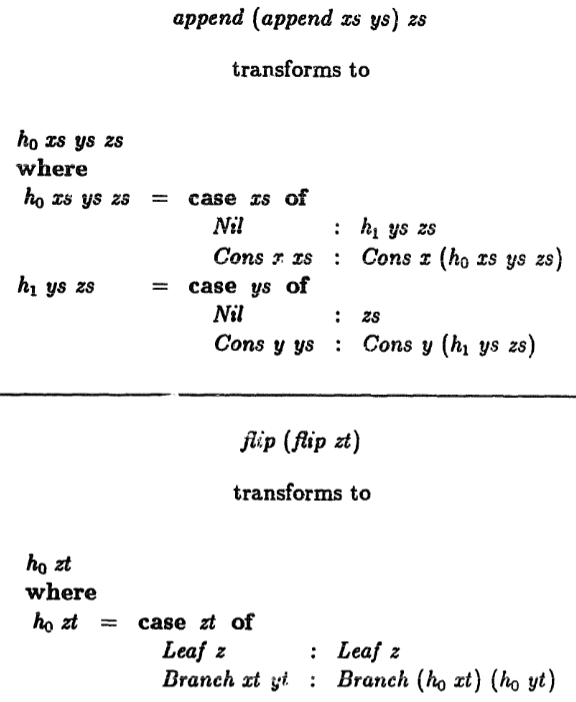
\includegraphics[width=0.55\textwidth]{figs/deforestation-examples}
    \caption{Примеры работы дефорестирующего алгоритма~\cite{wadler1988deforestation}.}
    \label{fig:deforestation-examples}
\end{figure}

Сфокусируемся на списках и рассмотрим более практичные решения\footnote{\url{https://markkarpov.com/tutorial/ghc-optimization-and-fusion.html}}.
Первым очевидным решением было бы для каждой пары функций, работающих со списками, добавить специальное правило переписывания (см.~\ref{subsubsec:rules}), дефорестирующее с помощью алгебраических свойств списочных трансформаций.
Однако, таких правил будет экспоненциально много.
\begin{minted}{haskell}
    {-# RULES
    "map/map" forall f g xs. map f (map g xs) = map (f . g) xs
      #-}
\end{minted}

Современная техника дефорестирования в Haskell --- fold/build list fusion~\cite{gill1993short} --- вместо использования множества алгебраических правил, определяет универсальный способ конструирования и деконструирования списка.
Деконструировать список будем с помощью \mintinline{haskell}|foldr|, и для него введём специальное правило:
\begin{minted}{haskell}
    foldr f ini . map g ?$\equiv$? foldr (f . g) ini
\end{minted}
Конструировать будем с помощью функции \mintinline{haskell}|build|:
\begin{minted}{haskell}
    build :: (forall b . (a -> b -> b) -> b -> b) -> [a]
    build g = g (:) []
\end{minted}
Например, список \mintinline{haskell}{[1, 2, 3]} и функция \mintinline{haskell}{map} теперь запишутся следующим образом\footnote{В стандартной библиотеке Haskell функции работы со списками написаны нормально, но рядом написаны правила \texttt{RULES}, которые подменяют их реализацию на fold/build.}:
\begin{minted}{haskell}
    list123 :: [Int]
    list123 = build \s z -> s 1 (s 2 (s 3 z))

    map :: (a -> b) -> [a] -> [b]
    map f xs = build \s z -> foldr (\x acc -> s (f x) acc) z xs
\end{minted}
Можно заметить, что на вход \texttt{build} передаётся список Чёрча, отсюда не удивителен закон:
\begin{minted}{haskell}
    foldr f ini (build g) ?$\equiv$? g f ini
\end{minted}

Таким образом, мы избавились от конструирования списков путём замены вызовов конструкторов на вызовы сворачивающих функций.

Дефорестацию также можно производить вручную (см.~\ref{fig:cpp-deforestation}).
\begin{figure}
    \centering
    \begin{tabular}{p{0.5\textwidth} rl}
        \begin{minipage}[t]{0.5\textwidth}
            \begin{minted}{cpp}
                std::variant<Msg1, Msg2>
                    deserialize(bytes bs) {
                    if (...) {
                        return std::variant{Msg1(...)};
                    else {
                        return std::variant{Msg2(...)};
                    }
                }
            \end{minted}
        \end{minipage}
        &
        \begin{minipage}[t]{0.5\textwidth}
            \begin{minted}{cpp}
                template<class Impl>
                auto deserialize(bytes bs) {
                    if (...) {
                        return Impl::processMsg1(...);
                    else {
                        return Impl::processMsg2(...);
                    }
                }
            \end{minted}
        \end{minipage}
    \end{tabular}
    \caption{Ручная дефорестация в C++.}
    \label{fig:cpp-deforestation}
\end{figure}

\subsubsection{Visitor pattern} \label{subsubsec:visitor}

Рассмотрим некоторое дерево и его свёртку:
\begin{minted}{haskell}
    data Tree a = Leaf | Node a [Tree a]
    foldTree :: Tree a -> r -> (a -> [r] -> r) -> r
\end{minted}

Перепишем и переименуем:
\begin{minted}{haskell}
    data Visitor a r = Visitor { onLeaf :: r, onNode :: a -> [r] -> r }
    visitTree :: Tree a -> Visitor a r -> r
\end{minted}

Чтобы это ещё более выглядело в ООП стиле, само дерево должно задаваться свёрткой (функцией \texttt{visit}), а разные вершины --- конкретными её реализациями:
\begin{minted}{haskell}
    type Tree a = forall r . Visitor a r -> r

    leaf :: Tree a
    leaf Visitor{onLeaf} = onLeaf

    node :: a -> [Tree a] -> Tree a
    node x ts v@Visitor{onNode} = onNode x (fmap ($ v) ts)
\end{minted}

\subsection{Всё --- развёртка} \label{subsec:all-unfolds}



% todo

\subsection{Вездесущий дуализм}

% todo
